\def\bmode{2} % Mode 0 for presentation, mode 1 (or not 0) for a handout with notes, mode 2 for handout without notes
\if 0\bmode
\documentclass[smaller]{beamer}
\else \if 1\bmode
\documentclass[smaller,handout]{beamer}
 \immediate\write18{pdflatex -jobname=\jobname-Notes-Handout\space\jobname}
\usepackage{handoutWithNotes}
\pgfpagesuselayout{2 on 1 with notes}[letterpaper, landscape, border shrink=4mm]
\else \if 2\bmode
\immediate\write18{pdflatex -jobname=\jobname-Handout\space\jobname}
\documentclass[smaller,handout]{beamer}
\fi
\fi
\fi


% \documentclass[smaller,handout
% ]{beamer}
%\usepackage{etex}
%\newcommand{\num}{6{} }

% \usetheme[
%   outer/progressbar=foot,
%   outer/numbering=counter,
%  block=fillFF
% ]{metropolis}

%\useoutertheme{metropolis}

\usetheme{Madrid}
\useoutertheme[subsection=false]{miniframes} % Alternatively: miniframes, infolines, split
\useinnertheme{circles}
\usecolortheme{seahorse}

\usepackage[backend=biber,style=authoryear,maxcitenames=2,maxbibnames=99,safeinputenc,url=false,
eprint=false]{biblatex}
\addbibresource{bib/references.bib}
\AtEveryCitekey{\iffootnote{{\tiny}\tiny}{\tiny}}

%\usepackage{pgfpages}
%\setbeameroption{hide notes} % Only slides
%\setbeameroption{show only notes} % Only notes
%\setbeameroption{hide notes} % Only notes
%\setbeameroption{show notes on second screen=right} % Both

% \usepackage[sfdefault]{Fira Sans}

% \setsansfont[BoldFont={Fira Sans}]{Fira Sans Light}
% \setmonofont{Fira Mono}

%\usepackage{fira}
%\setsansfont{Fira}
%\setmonofont{Fira Mono}
% To give a presentation with the Skim reader (http://skim-app.sourceforge.net) on OSX so
% that you see the notes on your laptop and the slides on the projector, do the following:
% 
% 1. Generate just the presentation (hide notes) and save to slides.pdf
% 2. Generate onlt the notes (show only nodes) and save to notes.pdf
% 3. With Skim open both slides.pdf and notes.pdf
% 4. Click on slides.pdf to bring it to front.
% 5. In Skim, under "View -> Presentation Option -> Synhcronized Noted Document"
%    select notes.pdf.
% 6. Now as you move around in slides.pdf the notes.pdf file will follow you.
% 7. Arrange windows so that notes.pdf is in full screen mode on your laptop
%    and slides.pdf is in presentation mode on the projector.

% Give a slight yellow tint to the notes page
%\setbeamertemplate{note page}{\pagecolor{yellow!5}\insertnote}\usepackage{palatino}


%\usetheme{metropolis}
%\usecolortheme{beaver}
%\usepackage{xcolor}
\definecolor{darkcandyapplered}{HTML}{A40000}
\definecolor{lightcandyapplered}{HTML}{e74c3c}

%\setbeamercolor{title}{fg=darkcandyapplered}
%\setbeamercolor{frametitle}{bg=darkcandyapplered!80!black!90!white}
%\setbeamertemplate{frametitle}{\bf\insertframetitle}
%\setbeamercolor{footnote mark}{fg=darkcandyapplered}
%\setbeamercolor{footnote}{fg=darkcandyapplered!70}
%\Raggedbottom
%\setbeamerfont{page number in head/foot}{size=\tiny}
%\usepackage[tracking]{microtype}


\setbeamertemplate{frametitle}{%
    \nointerlineskip%
    \begin{beamercolorbox}[wd=\paperwidth,ht=2.0ex,dp=0.6ex]{frametitle}
        \hspace*{1ex}\insertframetitle%
    \end{beamercolorbox}%
}



\setbeamerfont{caption}{size=\footnotesize}
\setbeamercolor{caption name}{fg=darkcandyapplered}


%\usepackage[sc,osf]{mathpazo}   % With old-style figures and real smallcaps.
%\linespread{1.025}              % Palatino leads a little more leading

% Euler for math and numbers
%\usepackage[euler-digits,small]{eulervm}
%\AtBeginDocument{\renewcommand{\hbar}{\hslash}}
\usepackage{graphicx,multirow,paralist,booktabs}


%\mode<presentation> { \setbeamercovered{transparent} }

\setbeamertemplate{navigation symbols}{}
\makeatletter
\def\beamerorig@set@color{%
  \pdfliteral{\current@color}%
  \aftergroup\reset@color
}
\def\beamerorig@reset@color{\pdfliteral{\current@color}}
\makeatother

%=== GRAPHICS PATH ===========
\graphicspath{{./m3-images/}}
% Marginpar width
%Marginpar width
%\setlength{\marginparsep}{.02in}


%% Captions
% \usepackage{caption}
% \captionsetup{
%   labelsep=quad,
%   justification=raggedright,
%   labelfont=sc
% }

%AMS-TeX packages

\usepackage{amssymb,amsmath,amsthm} 
\usepackage{bm}
\usepackage{color}

\usepackage{hyperref,enumerate}
\usepackage{minitoc,array}


%https://tex.stackexchange.com/a/31370/2269
\usepackage{mathtools,cancel}

\renewcommand{\CancelColor}{\color{red}} %change cancel color to red

\makeatletter
\let\my@cancelto\cancelto %copy over the original cancelto command
\newcommand<>{\cancelto}[2]{\alt#3{\my@cancelto{#1}{#2}}{\mathrlap{#2}\phantom{\my@cancelto{#1}{#2}}}}
% redefine the cancelto command, using \phantom to assure that the
% result doesn't wiggle up and down with and without the arrow
\makeatother


\definecolor{slblue}{rgb}{0,.3,.62}
\hypersetup{
    colorlinks,%
    citecolor=blue,%
    filecolor=blue,%
    linkcolor=blue,
    urlcolor=slblue
}

%%% TIKZ
\usepackage{animate}
\usepackage{tikz}
\usepackage{pgfplots}
\usepackage{pgfplotstable}
\usepackage{pgfgantt}
\usepackage{tikzsymbols}
\pgfplotsset{compat=newest}
\usepgfplotslibrary{groupplots,fillbetween}

\usetikzlibrary{arrows,shapes,positioning,shapes.geometric}
\usetikzlibrary{decorations.markings}
\usetikzlibrary{shadows,automata}
\usetikzlibrary{patterns,matrix}
\usetikzlibrary{trees,mindmap,backgrounds}
%\usetikzlibrary{circuits.ee.IEC}
\usetikzlibrary{decorations.text}
% For Sagnac Picture
\usetikzlibrary{%
    decorations.pathreplacing,%
    decorations.pathmorphing%
}
\tikzset{no shadows/.style={general shadow/.style=}}
%
%\usepackage{paralist}



%%% FORMAT PYTHON CODE
%\usepackage{listings}
% Default fixed font does not support bold face
\DeclareFixedFont{\ttb}{T1}{txtt}{bx}{n}{8} % for bold
\DeclareFixedFont{\ttm}{T1}{txtt}{m}{n}{8}  % for normal

% Custom colors
\definecolor{deepblue}{rgb}{0,0,0.5}
\definecolor{deepred}{rgb}{0.6,0,0}
\definecolor{deepgreen}{rgb}{0,0.5,0}

%\usepackage{listings}

% Python style for highlighting
% \newcommand\pythonstyle{\lstset{
% language=Python,
% basicstyle=\footnotesize\ttm,
% otherkeywords={self},             % Add keywords here
% keywordstyle=\footnotesize\ttb\color{deepblue},
% emph={MyClass,__init__},          % Custom highlighting
% emphstyle=\footnotesize\ttb\color{deepred},    % Custom highlighting style
% stringstyle=\color{deepgreen},
% frame=tb,                         % Any extra options here
    % showstringspaces=false            % 
% }}

% % Python environment
% \lstnewenvironment{python}[1][]
% {
% \pythonstyle
% \lstset{#1}
% }
% {}

% % Python for external files
% \newcommand\pythonexternal[2][]{{
% \pythonstyle
% \lstinputlisting[#1]{#2}}}

% Python for inline
% 
% \newcommand\pythoninline[1]{{\pythonstyle\lstinline!#1!}}


\newcommand{\osn}{\oldstylenums}
\newcommand{\dg}{^{\circ}}
\newcommand{\lt}{\left}
\newcommand{\rt}{\right}
\newcommand{\pt}{\phantom}
\newcommand{\tf}{\therefore}
\newcommand{\?}{\stackrel{?}{=}}
\newcommand{\fr}{\frac}
\newcommand{\dfr}{\dfrac}
\newcommand{\ul}{\underline}
\newcommand{\tn}{\tabularnewline}
\newcommand{\nl}{\newline}
\newcommand\relph[1]{\mathrel{\phantom{#1}}}
\newcommand{\cm}{\checkmark}
\newcommand{\ol}{\overline}
\newcommand{\rd}{\color{red}}
\newcommand{\bl}{\color{blue}}
\newcommand{\pl}{\color{purple}}
\newcommand{\og}{\color{orange!90!black}}
\newcommand{\gr}{\color{green!40!black}}
\newcommand{\nin}{\noindent}
\newcommand{\la}{\lambda}
\renewcommand{\th}{\theta}
\newcommand{\al}{\alpha}
\newcommand{\G}{\Gamma}
\newcommand*\circled[1]{\tikz[baseline=(char.base)]{
            \node[shape=circle,draw,thick,inner sep=1pt] (char) {\small #1};}}

\newcommand{\bc}{\begin{compactenum}[\quad--]}
\newcommand{\ec}{\end{compactenum}}

\newcommand{\p}{\partial}
\newcommand{\pd}[2]{\frac{\partial{#1}}{\partial{#2}}}
\newcommand{\dpd}[2]{\dfrac{\partial{#1}}{\partial{#2}}}
\newcommand{\pdd}[2]{\frac{\partial^2{#1}}{\partial{#2}^2}}


\pgfmathdeclarefunction{poiss}{1}{%
  \pgfmathparse{(#1^x)*exp(-#1)/(x!)}%
  }

\pgfmathdeclarefunction{gauss}{2}{%
  \pgfmathparse{1/(#2*sqrt(2*pi))*exp(-((x-#1)^2)/(2*#2^2))}%
}

\pgfmathdeclarefunction{expo}{2}{%
  \pgfmathparse{#1*exp(-#1*#2)}%
}

\pgfmathdeclarefunction{expocdf}{2}{%
  \pgfmathparse{1 -exp(-#1*#2)}%
}

\makeatletter
\long\def\ifnodedefined#1#2#3{%
    \@ifundefined{pgf@sh@ns@#1}{#3}{#2}%
}

\pgfplotsset{
    discontinuous/.style={
    scatter,
    scatter/@pre marker code/.code={
        \ifnodedefined{marker}{
            \pgfpointdiff{\pgfpointanchor{marker}{center}}%
             {\pgfpoint{0}{0}}%
             \ifdim\pgf@y>0pt
                \tikzset{options/.style={mark=*, fill=white}}
                \draw [densely dashed] (marker-|0,0) -- (0,0);
                \draw plot [mark=*] coordinates {(marker-|0,0)};
             \else
                \tikzset{options/.style={mark=none}}
             \fi
        }{
            \tikzset{options/.style={mark=none}}        
        }
        \coordinate (marker) at (0,0);
        \begin{scope}[options]
    },
    scatter/@post marker code/.code={\end{scope}}
    }
}

\makeatother

\renewcommand{\arraystretch}{1.5}
%%%%%%%%%%%%%%%%%%%%%%%%%%%%%%%%%%%%%%%%%%%%%%%%%%%
%%%%%%%%%%%%%%%%%%%%%%%%%%%%%%%%%%%%%%%%%%%%%%%%%%%

\title[CEE 260/MIE 273 3f: Joint Distributions]{{\normalsize CEE 260/MIE 273: Probability and Statistics in Civil Engineering} \\
Lecture 3f: Joint Distributions }
\date[\today]{\footnotesize \today}
\author{{\bf Prof.\ Oke}}
\institute[UMass Amherst]{
  \begin{tikzpicture}[baseline=(current bounding box.center)]
    \node[anchor=base] at (-7,0) (its) {
\includegraphics[scale=.3]{UMassEngineering_vert}} ;
  \end{tikzpicture}
}



%https://tex.stackexchange.com/questions/55806/mindmap-tikzpicture-in-beamer-reveal-step-by-step
  % \tikzset{
  %   invisible/.style={opacity=0},
  %   visible on/.style={alt={#1{}{invisible}}},
  %   alt/.code args={<#1>#2#3}{%
  %     \alt<#1>{\pgfkeysalso{#2}}{\pgfkeysalso{#3}} % \pgfkeysalso doesn't change the path
  %   },
  % }


\usepackage{listings}

\lstset{language=matlab,
                basicstyle=\scriptsize\ttfamily,
                keywordstyle=\color{blue}\ttfamily,
                stringstyle=\color{blue}\ttfamily,
                commentstyle=\color{gray}\ttfamily,
                morecomment=[l][\color{gray}]{\#}
              }
         
\begin{document}

\maketitle




\begin{frame}
  \frametitle{Outline}
  \tableofcontents
\end{frame}
 
\section{Preamble}
 

\begin{frame}
  \frametitle{Today's objectives}
  \pause

  Joint distributions: \pause

  \begin{itemize}
  \item Understand the concept of jointly distributed random variables \pause
  \item Differentiate between marginal and conditional distributions \pause
  \item Manipulate joint distributions to compute probabilities
   \end{itemize}
\end{frame}


\section{Joint distributions}

\begin{frame}
  \frametitle{Joint distributions}\pause
  Given two random variables $X$ and $Y$:

  \begin{block}{Discrete case}
    The joint PMF is:
    \begin{equation}
      \label{eq:62}
      p_{X,Y}(x_i,y_j) = P(X=x_i, Y = y_j)
    \end{equation} \pause
    The CDF is:
    \begin{equation}
      \label{eq:63}
      F_{X,Y}(x,y) = \sum_{x_i \le x}\sum_{y_j \le y} p_{X,Y}(x_i, y_j)
    \end{equation}
  \end{block}
  \pause

  \begin{block}{Continuous case}\pause
    The joint probability is given by:
    \begin{equation}
      P(a < X \le b, c < Y \le d) = \int_a^b \int_c^d f_{X,Y}(x,y)dy dx
    \end{equation}
  \end{block}
\end{frame}

\begin{frame}
  \frametitle{Joint and marginal distributions} \pause

  Marginal distributions: $f(x_1)$ and  $f(x_2)$ \\ \pause
  Joint distribution: $f(x_1,x_2)$. \pause
  
  \pgfplotsset{
    colormap={whitered}{color(0cm)=(white); color(1cm)=(purple!75!blue)}
  }

  \begin{tikzpicture}[scale=.6,
    declare function={mu1=1;},
    declare function={mu2=2;},
    declare function={sigma1=0.5;},
    declare function={sigma2=1;},
    declare function={normal(\m,\s)=1/(2*\s*sqrt(pi))*exp(-(x-\m)^2/(2*\s^2));},
    declare function={bivar(\ma,\sa,\mb,\sb)=
      1/(2*pi*\sa*\sb) * exp(-((x-\ma)^2/\sa^2 + (y-\mb)^2/\sb^2))/2;}]
    \begin{axis}[
      colormap name=whitered,
      width=15cm,
      view={45}{65},
      enlargelimits=false,
      grid=major,
      domain=-1:4,
      y domain=-1:4,
      samples=26,
      xlabel=$x_1$,
      ylabel=$x_2$,
      zlabel={$P$},
      colorbar,
      colorbar style={
        at={(1.1,0)},
        anchor=south west,
        height=0.25*\pgfkeysvalueof{/pgfplots/parent axis height},
        title={$P(x_1,x_2)$}
      }
      ]
      \only<4->{\addplot3 [domain=-1:4,samples=31, samples y=0, red, thick, smooth] (x,4,{normal(mu1,sigma1)});
      \addplot3 [domain=-1:4,samples=31, samples y=0, blue, thick, smooth] (-1,x,{normal(mu2,sigma2)});
      \addplot3 [surf] {bivar(mu1,sigma1,mu2,sigma2)};}

      \only<5->{\draw [black!50] (axis cs:-1,0,0) -- (axis cs:4,0,0);}
      \only<6->{\draw [black!50] (axis cs:0,-1,0) -- (axis cs:0,4,0);}

      \only<8->{\node[blue] at (axis cs:-1,1,0.18) [pin=165:$f(x_2)$] {};}
      \only<7->{\node[red] at (axis cs:1.5,4,0.32) [pin=-15:$f(x_1)$] {};}
    \end{axis}
  \end{tikzpicture}
\end{frame}


% \begin{frame}
%   \frametitle{Covariance and correlation}
%   Recall that the variance of an r.v.\ $X$ is given by:
%   \begin{equation}
%     \label{eq:52}
%     Var(X) = E[(X-\mu_X)^2 ] = E(X^2) - E(X)^2
%   \end{equation}

%   Then given two r.v.'s $X$ and $Y$, the {\it covariance} measures the strength of the linear relationship between them.
%   \pause
  
%   \begin{block}{Covariance}
%     \begin{equation}
%       \label{eq:50}
%       Cov(X,Y) = E[(X-\mu_X)(Y-\mu_Y)] = E(XY) - E(X)E(Y)
%     \end{equation}    
%   \end{block}

% \pause

%   \begin{block}{Correlation coefficient}
%     This is the normalized covariance
%     \begin{equation}
%     \label{eq:51}
%     \rho = \fr{Cov(X,Y)}{\sigma_X\sigma_Y}
%   \end{equation}
%   \end{block}
    
% \end{frame}

\section{Discrete random variables}
\begin{frame}
  \frametitle{Example 1: Joint PMF of two random variables}
  \pause
  Given two random variables $X$ and $Y$ with joint PMF indicated in the table below:
  \pause

  \begin{center}
    \begin{tabular}{c | c | c | c | c}
            & $Y=0$ & $Y=1$ & $Y=2$  & $p_{X}(x)$\\\hline
      $X=0$ & $\fr16$ & $\fr14$ & $\fr18$ & ? \\\hline
      $X=1$ & $\fr18$ & $\fr16$ & $\fr16$ & ? \\\hline
      $p_{Y}(y)$ & ? & ? & ? 
    \end{tabular}
  \end{center}
  \pause

  \begin{center}
    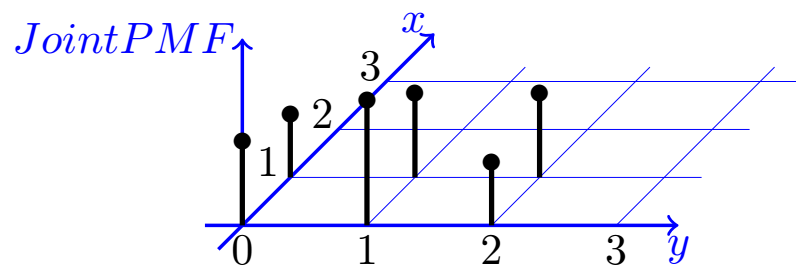
\includegraphics[width=.6\textwidth]{jointpmf}
  \end{center}
  \pause
  
  \begin{enumerate}[\bf(a)]
  \item Find $P(X=0,Y\le 1)$ \pause
  \item Find the marginal PMFs of $X$ and $Y$
  \item Find $P(Y=1| X=0)$
  \item Are $X$ and $Y$ independent?
  \end{enumerate}
\end{frame}

\begin{frame}
  \frametitle{Example 1: Joint PMF of two random variables (cont.)}

  \pause

  

  \begin{exampleblock}{Solution}
    \begin{enumerate}[\bf(a)]\setcounter{enumi}{0}
    \item To find the probability $P(X = 0 , Y \le 1)$, simply add up the cells \textit{jointly} satisfying the conditions. \pause

          \begin{center}
    \begin{tabular}{c | c | c | c | c}
            & $Y=0$ & $Y=1$ & $Y=2$  & $p_{X}(x)$\\\hline
      $X=0$ & \rd $\fr16$ &\rd $\fr14$ & $\fr18$ & ? \\\hline
      $X=1$ & $\fr18$ & $\fr16$ & $\fr16$ & ? \\\hline
      $p_{Y}(y)$ & ? & ? & ? 
    \end{tabular}
  \end{center}
  
      \begin{eqnarray*}
        P(X = 0 , Y \le 1) &=& \pause \fr 16 + \fr14 \\ \pause
                           &=& \fr{4 + 6}{24} = \fr{10}{24} \pause = \fr{5}{12}
      \end{eqnarray*}
    \end{enumerate}
  \end{exampleblock}
\end{frame}


\begin{frame}
  \frametitle{Example 1: Joint PMF of two random variables (cont.)}

  \pause

  \begin{exampleblock}{Solution}
    \begin{enumerate}[\bf(a)]\setcounter{enumi}{1}
    \item To find the marginal PMFs of $X$ and $Y$, i.e.\ $p_{X}(x) = P(X=x)$ and $p_{Y}(y) =P(Y=y)$, respectively, sum up the rows and columns in the table: \pause
          \begin{center}
    \begin{tabular}{c | c | c | c | c}
            & $Y=0$ & $Y=1$ & $Y=2$  & \bl $p_{X}(x)$\\\hline
      $X=0$ & $\fr16$ & $\fr14$ & $\fr18$ & \pause \bl $\fr 16 + \fr14 + \fr18 \pause = \fr{13}{24}$ \\\hline \pause
      $X=1$ & $\fr18$ & $\fr16$ & $\fr16$ & \pause \bl $\fr 18 + \fr16 + \fr16 \pause = \fr{11}{24}$ \\\hline \pause
      \rd $p_{Y}(y)$
            & \pause \rd $\fr16 + \fr18 = \pause \fr{7}{24}$\pause
                      & \rd $\fr14 + \fr16 = \pause \fr{5}{12}$ \pause
                                & \rd $\fr18 + \fr16 = \pause \fr{7}{24}$
    \end{tabular}
  \end{center}
  \pause
  Thus, we obtain:
  
  \begin{minipage}{.45\linewidth}\bl
    \pause
    \begin{eqnarray*}
      p_{X}(x) = \pause
      \begin{cases}
        \fr{13}{24}, & x = 0 \\\pause
        \fr{11}{24}, & x = 1 \\\pause
        0, & \text{otherwise}
      \end{cases}
    \end{eqnarray*}
  \end{minipage}
  \pause
  \begin{minipage}{.45\linewidth}\rd
        \pause
    \begin{eqnarray*}
      p_{Y}(y) = \pause
      \begin{cases}
        \fr{7}{24}, & y = 0 \\\pause
        \fr{5}{12}, & y = 1 \\\pause
        \fr{7}{24}, & y = 2 \\\pause
        0,          & \text{otherwise}
      \end{cases}
    \end{eqnarray*}
  \end{minipage}
    \end{enumerate} 
  \end{exampleblock}
\end{frame}


\begin{frame}
  \frametitle{Example 1: Joint PMF of two random variables (cont.)}

  \pause

            \begin{center}
    \begin{tabular}{c | c | c | c | c}
            & $Y=0$ & $Y=1$ & $Y=2$  & \bl $p_{X}(x)$\\\hline
      $X=0$ & $\fr16$ & $\fr14$ & $\fr18$ &  \bl $\fr 16 + \fr14 + \fr18 \pause = \fr{13}{24}$ \\\hline  
      $X=1$ & $\fr18$ & $\fr16$ & $\fr16$ &  \bl $\fr 18 + \fr16 + \fr16 \pause = \fr{11}{24}$ \\\hline  
      \rd $p_{Y}(y)$
            &  \rd $\fr16 + \fr18 = \pause \fr{7}{24}$ 
                      & \rd $\fr14 + \fr16 = \pause \fr{5}{12}$  
                                & \rd $\fr18 + \fr16 = \pause \fr{7}{24}$
    \end{tabular}
  \end{center}
  \pause
  
  \begin{exampleblock}{Solution}
    \begin{enumerate}[\bf(a)]\setcounter{enumi}{2}
    \item Here we use the conditional probability formula: \pause
      \begin{eqnarray*}
        P(Y = 1 | X = 0) &=& \pause \fr{P(Y = 1 \cap X = 0)}{P(X = 0)} \pause = \fr{P(Y = 1, X = 0)}{P(X = 0)} \\\pause
                         &=& \fr{p_{XY}(0,1)}{p_{X}(0)} =  \pause
                         \fr{\fr14}{\fr{13}{24}} = \pause \fr{6}{13}                             
      \end{eqnarray*}


    \end{enumerate}
  \end{exampleblock}
\end{frame}

\begin{frame}
  \frametitle{Example 1: Joint PMF of two random variables (cont.)}

  \pause

            \begin{center}
    \begin{tabular}{c | c | c | c | c}
            & $Y=0$ & $Y=1$ & $Y=2$  & \bl $p_{X}(x)$\\\hline
      $X=0$ & $\fr16$ & $\fr14$ & $\fr18$ &  \bl $\fr 16 + \fr14 + \fr18 \pause = \fr{13}{24}$ \\\hline  
      $X=1$ & $\fr18$ & $\fr16$ & $\fr16$ &  \bl $\fr 18 + \fr16 + \fr16 \pause = \fr{11}{24}$ \\\hline  
      \rd $p_{Y}(y)$
            &  \rd $\fr16 + \fr18 = \pause \fr{7}{24}$ 
                      & \rd $\fr14 + \fr16 = \pause \fr{5}{12}$  
                                & \rd $\fr18 + \fr16 = \pause \fr{7}{24}$
    \end{tabular}
  \end{center}
  \pause
  \begin{exampleblock}{Solution}
    \begin{enumerate}[\bf(a)]\setcounter{enumi}{3}

    \item Two r.v.'s are independent if $P(Y = y_{j}|X = x_{i}) = P(X=x_{i})$ or $P(X=x_{i}|Y=y_{j}) = P(Y=y_{j})$ for all $i$ and $j$.
      \pause
      Here,
      \begin{equation*}
        P(Y=1|X=0) \pause = \fr{6}{13} \pause \ne P(Y=1)\pause = \fr{5}{12}
      \end{equation*}
      The independence condition fails. \pause Hence $X$ and $Y$ are not independent.
    \end{enumerate}
  \end{exampleblock}
\end{frame}

\section{Continuous random variables}
 
\begin{frame}
  \frametitle{Conditional distributions of continuous random variables}
  Recall the definition of conditional probability (multiplication rule):\pause
  \begin{eqnarray}
    P(A|B) &=& \fr{P(AB)}{P(B)} \\\pause
    P(AB) &=& \pause P(A|B)P(B)  = \pause P(B|A)P(A)
  \end{eqnarray}
  \pause
  Similarly, for two continuous r.v.'s, the conditional PDF of $X$ given $Y$ is:
  \begin{equation}
    \label{eq:10}
    f_{X|Y}(x|y) = \fr{f_{X,Y}(x,y)}{f_Y(y)}
  \end{equation}
  \pause
  \begin{block}{Joint PDF and CDF of two variables}\pause
  The joint PDF is given by:
  \begin{equation}
    \label{eq:11}
    f_{X,Y}(x,y) = f_{X|Y}(x|y)f_Y(y) = f_{Y|X}(y|x)f_X(x)
  \end{equation}
  \pause
  While the joint CDF is given by:
   \begin{equation}
    \label{eq:13}
    F_{X,Y}(a,b) = P(X\le a,Y\le b) =\pause \int_{-\infty}^a \int_{-\infty}^b f_{X,Y}(x,y)dydx
  \end{equation}
\end{block}
\end{frame}

\begin{frame}
  \frametitle{Marginal distributions of continuous random variables} \pause
  Recall the theorem of total probability:\pause
  \begin{equation}
    \label{eq:12}
    P(A) = \pause \sum_{i=1}^n \pause P(A|E_i) \pause P(E_i)
  \end{equation}
  \pause
  Similarly, the marginal PDFs from a joint distribution of two continuous r.v.'s $X$ and $Y$ is given as:\pause
  \begin{eqnarray}
    f_X(x) &=& \pause \int_{-\infty}^\infty f_{X|Y}(x|y)f_Y(y)dy =\pause \int_{-\infty}^\infty f_{X,Y}(x,y)dy \\ \pause
    f_Y(y) &=&\pause \int_{-\infty}^\infty f_{Y|X}(y|x)f_X(x)dx =\pause  \int_{-\infty}^\infty f_{X,Y}(x,y)dx
  \end{eqnarray}
\end{frame}

\begin{frame}
  \frametitle{Example 2: Water levels}\pause
    The daily water levels of two reservoirs A and B are denoted by two r.v.'s $X$ and $Y$ having the following joint PDF:\pause
    \begin{equation*}
      f(x,y) = \fr65\lt(x  + y^2\rt), \quad 0 < x < 1; 0 < y< 1
    \end{equation*}
    \begin{enumerate}[(a)]
    \item Determine the marginal density function of the daily water level for reservoir A.
    \item If reservoir A is half full on a given day, what is the probability that the water level will be more than half full?
    \end{enumerate}
 \end{frame}

\begin{frame}
  \frametitle{Example 2: Water levels (cont.)}\pause
      \begin{equation*}
      f(x,y) = \fr65\lt(x  + y^2\rt), \quad 0 < x < 1; 0 < y< 1
    \end{equation*}
    
  \begin{exampleblock}{Solution}
    \begin{enumerate}[(a)]
    \item We obtain the marginal density function $f_X(x)$ by integrating the joint PDF over $y$:\pause
      \begin{eqnarray*}
        f_X(x) &=& \int_0^1\fr65\lt(x+y^2\rt)dy  \\\pause
               &=& \fr65\lt[xy + \fr{y^3}{3}\rt]_0^1 \\\pause
               &=& \fr25\lt(3x + 1\rt) \quad (0 < x < 1)
      \end{eqnarray*}
    \end{enumerate}
  \end{exampleblock}

    \pause

    This is the \textbf{marginal distribution}
 \end{frame}


\begin{frame}
  \frametitle{Example 2: Water levels (cont.)}\pause

  \begin{equation*}
    f(x,y) = \fr65\lt(x  + y^2\rt), \quad 0 < x < 1; 0 < y< 1
  \end{equation*}
  
  \begin{exampleblock}{Solution}
    \begin{enumerate}[(a)]\setcounter{enumi}{1}
    \item {\gr If reservoir A is half full on a given day, what is the probability that the water level will be more than half full?} \pause
      We first find the conditional distribution:\pause
      \begin{eqnarray*}
        f_{Y|X}(y|x) &=& \fr{f_{X,Y}(x,y)}{f_X(x)} = \pause \fr{\fr65\lt(x+y^2\rt)}{\fr25\lt(3x + 1\rt)^2} \pause = 3\fr{x+y^2}{3x +1}\\\pause
        \text{Thus: } P(Y > 0.5 | X = 0.5) &=& \pause \int_{0.5}^1f_{Y|X}(y|x=0.5)dy \\\pause
                     &=&3\int_{0.5}^1\fr{0.5+y^2}{1.5 + 1} dy \\\pause
                     &=& \lt(\fr3{2.5}\rt)\pause \lt[0.5y + \fr{y^3}{3}\rt]_{0.5}^1 \pause
                     = \boxed{\gr 0.65}
      \end{eqnarray*}
    \end{enumerate}
  \end{exampleblock}

 \end{frame}

 \begin{frame}
   \frametitle{Reading}
   \pause

   \begin{itemize}[<+->]
   \item Exponential distribution: Section 4.7 (Navidi)

   \item {\rd Also read up on the Uniform Distribution in Section 4.8 (Navidi)}
     
   \item Joint distributions: Section 2.6 (Navidi)
   \end{itemize}
 \end{frame}

% \begin{frame}
%   \frametitle{MATLAB Homework}
%   \pause

%   \begin{itemize}
%   \item Ensure your submission is strictly a script saved with the \texttt{\rd .m} extension
%     \pause
%     \medskip
    
%   % \item Subsequent templates will include \texttt{clc} and \texttt{clear all} at the beginning of the script to facilitate grading by the TA
%   %   \pause
%   %   \medskip
    
%   \item MATLAB can only execute a script if it is in the \textit{\rd current folder}. \pause Otherwise you may get a message like the one below:
%     \pause 
%     \begin{center}
%       
\includegraphics[width=.4\textwidth]{matlab}
%     \end{center}
%     \pause
%     If so, simply click on \texttt{Change Folder} or move the file to the current folder you are in. Finally, always make sure the path of a file being read by a script is valid from its location, otherwise you will have to deal with ``File not found'' errors.

%     \pause
%     \medskip

%   \item MATLAB Homework 2 is due October 20, midnight.
%   \end{itemize}
% \end{frame}


% \begin{frame}
%   \frametitle{Midterm Exam}
%   \pause

%   \begin{itemize}
%   \item 24-hour open-resource examination
%     \pause

%     \medskip
    
%   \item Available for download via Moodle on Tuesday, October 19th at \textbf{10:00 AM}\pause
%     \medskip

%   \item Due by October 23rd at \textbf{11:59 PM}\pause
%     \medskip

%   \item Exam length will be similar to last year's midterm or the practice exam(s) available on Moodle.
%     \pause
%     \medskip
    
%   \item Exam is designed to be completed in 2-3 hours or less. \pause The 24-hr window gives you flexibility and time to
%     plan, organize and check your work before submission.
%     \pause
%     \medskip

%   \item You will be allowed to use your calculator or Matlab to compute probabilities (as long as you indicate how you obtained your answer).
%     \pause
%     \medskip
    
% %  \item \bl Next lecture (Tuesday, October 6th) will be a \textbf{Midterm Review Session}
%   \end{itemize}
% \end{frame}

% \begin{frame}
%   \frametitle{Continuous marginal and conditional distributions in practice}
%   \begin{exampleblock}{Example 1: Water levels}
%     \begin{enumerate}[(a)]
%     \end{enumerate}
%   \end{exampleblock}
% \end{frame}

% \begin{frame}
%   \frametitle{Functions of multiple random variables: key implications}\pause
  
%   \begin{block}{(1) The sum of independent Poisson processes is  a Poisson process}\pause
%     If $Z = \sum_{i=1}^n X_i$, where $X_i\sim \text{Poisson}(v_i)$, then:
%     \begin{equation}
%       \label{eq:21}
%     v_Z= \sum_{i=1}^n v_i
%   \end{equation}
%   \end{block}

%   \pause
  
%   \begin{block}{(2) The sum/difference of independent normal variates is normal} \pause
%     If $Z  = \sum_{i=1}^n a_i X_i$, then $\mu_Z = \sum_{i=1}^na_i\mu_{X_i}$ and $\sigma_Z^2 = \sum_{i=1}^n a_i^2\sigma_{X_i}^2$ \pause
%   \end{block}

  
% \end{frame}

% \begin{frame}
%   \frametitle{Functions of multiple random variables: key implications}\pause
% \begin{block}{(3) The quotient/product of independent lognormal variates is lognormal}\pause
%     If $Z = \prod_{i=1}^nX_i$, where $X_i \sim \text{Lognormal}(\la_{X_i},\zeta_{X_i})$, then\pause
%     \begin{equation}
%       \label{eq:22}
%       \la_Z = \sum_{i=1}^n\la_{X_i} \quad \zeta_Z^2 = \sum_{i=1}^n\zeta_{X_i}^2
%     \end{equation}
%   \end{block}

% \end{frame}


% \section{Outlook}
% \begin{frame}
%   \frametitle{Recap}
%   \begin{itemize}
%   \item \textbf{Lognormal distribution:} $X\sim LN(\mu,\sigma^{2})$\\
%     CDF: $F_{X}(x) = P(X\le x) = \Phi((\ln(x) - \mu)/\sigma)$\\\pause
%     \pause
%     Mean:
%     \begin{equation}
%       \label{eq:15}
%       E(X) = e^{\lt(\mu + \fr12 \sigma^2\rt)}
%     \end{equation}
%     \pause    
%     Variance:
%       \begin{equation}
%     \label{eq:16}
%     Var(X) = \pause   (e^{\sigma^2} - 1)e^{(2\mu + \sigma^{2})}
%   \end{equation}
    
%   \item \textbf{Exponential distribution}: $X \sim Exp(\la)$
%     \pause
%     \begin{eqnarray}
%       \text{PDF:}\quad  f_{X}(x) &=& \pause \la e^{-\la x}, \pause \qquad x > 0 \\
%       \text{CDF:}\quad  F_{X}(x) &=& P(X \le x) = \pause  1 - e^{-\la x}, \pause \qquad x > 0 
%     \end{eqnarray}

%     \pause

%     Mean:
%     \begin{equation}
%       E(X) = \fr{1}{\la}
%     \end{equation}

%     \pause

%     Variance:
%     \begin{equation}
%       Var(X) = \fr{1}{\la^{2}}
%     \end{equation}
%   \end{itemize}
% \end{frame}


%\begin{frame}[allowframebreaks]
%   \frametitle{References}
%   \AtNextBibliography{\scriptsize}
%   \setbeamertemplate{bibliography item}[text]
%   \printbibliography[heading=none]
  
% \end{frame}

%\printbibliography
\end{document}
%%% Local Variables:
%%% mode: latex
%%% TeX-master: t
%%% End:
